\documentclass[12pt,a4paper]{article}
\usepackage[utf8]{inputenc}
\usepackage[T2A]{fontenc}
\usepackage[russian]{babel}
\usepackage{amsmath}
\usepackage{graphicx}
\usepackage{geometry}
\usepackage{indentfirst}
\usepackage{float}
\usepackage{booktabs}

\geometry{left=2.5cm, right=1.5cm, top=2cm, bottom=2cm}
\graphicspath{{photoes/}}

\newcommand{\COO}{\mathrm{CO_2}}

\begin{document}

\begin{titlepage}
    \begin{center}
        \textbf{МОСКОВСКИЙ ФИЗИКО-ТЕХНИЧЕСКИЙ ИНСТИТУТ} \\
        \textbf{(НАЦИОНАЛЬНЫЙ ИССЛЕДОВАТЕЛЬСКИЙ УНИВЕРСИТЕТ)}
        \\[1cm]
        {\large Физтех-школа аэрокосмических технологий}
        \\[3.5cm]
        {\Huge \textbf{Определение времени колебательной релаксации CO$_2$}}
        \\[0.5cm]
        {\large Лабораторная работа №\,13 (Л.р.\,16 практикума)}
        \\[1.5cm]
        \begin{flushright}
            \begin{tabular}{l l}
                Ларькин Глеб & Б03-301 \\
            \end{tabular}
        \end{flushright}
        \vfill
        {\large Долгопрудный, 2026 г.}
    \end{center}
\end{titlepage}

\section{Цель работы}

Определить время колебательно-поступательной релаксации CO$_2$ методом
Кантровица при 24 и 65\,$^\circ$C, сравнить результаты с данными
практикума и оценить нагрев газа в ресивере.

\section{Установка и метод}

Газ из ресивера с давлением $p_0$ и температурой $T_0$ выходит
через дозвуковое сопло в атмосферу. Трубка Пито на оси струи
тормозит поток и измеряет полное давление $p_2$. Водяной дифманометр
измеряет перепад $\Delta p=p_0-p_2$.

\begin{figure}[H]
\centering
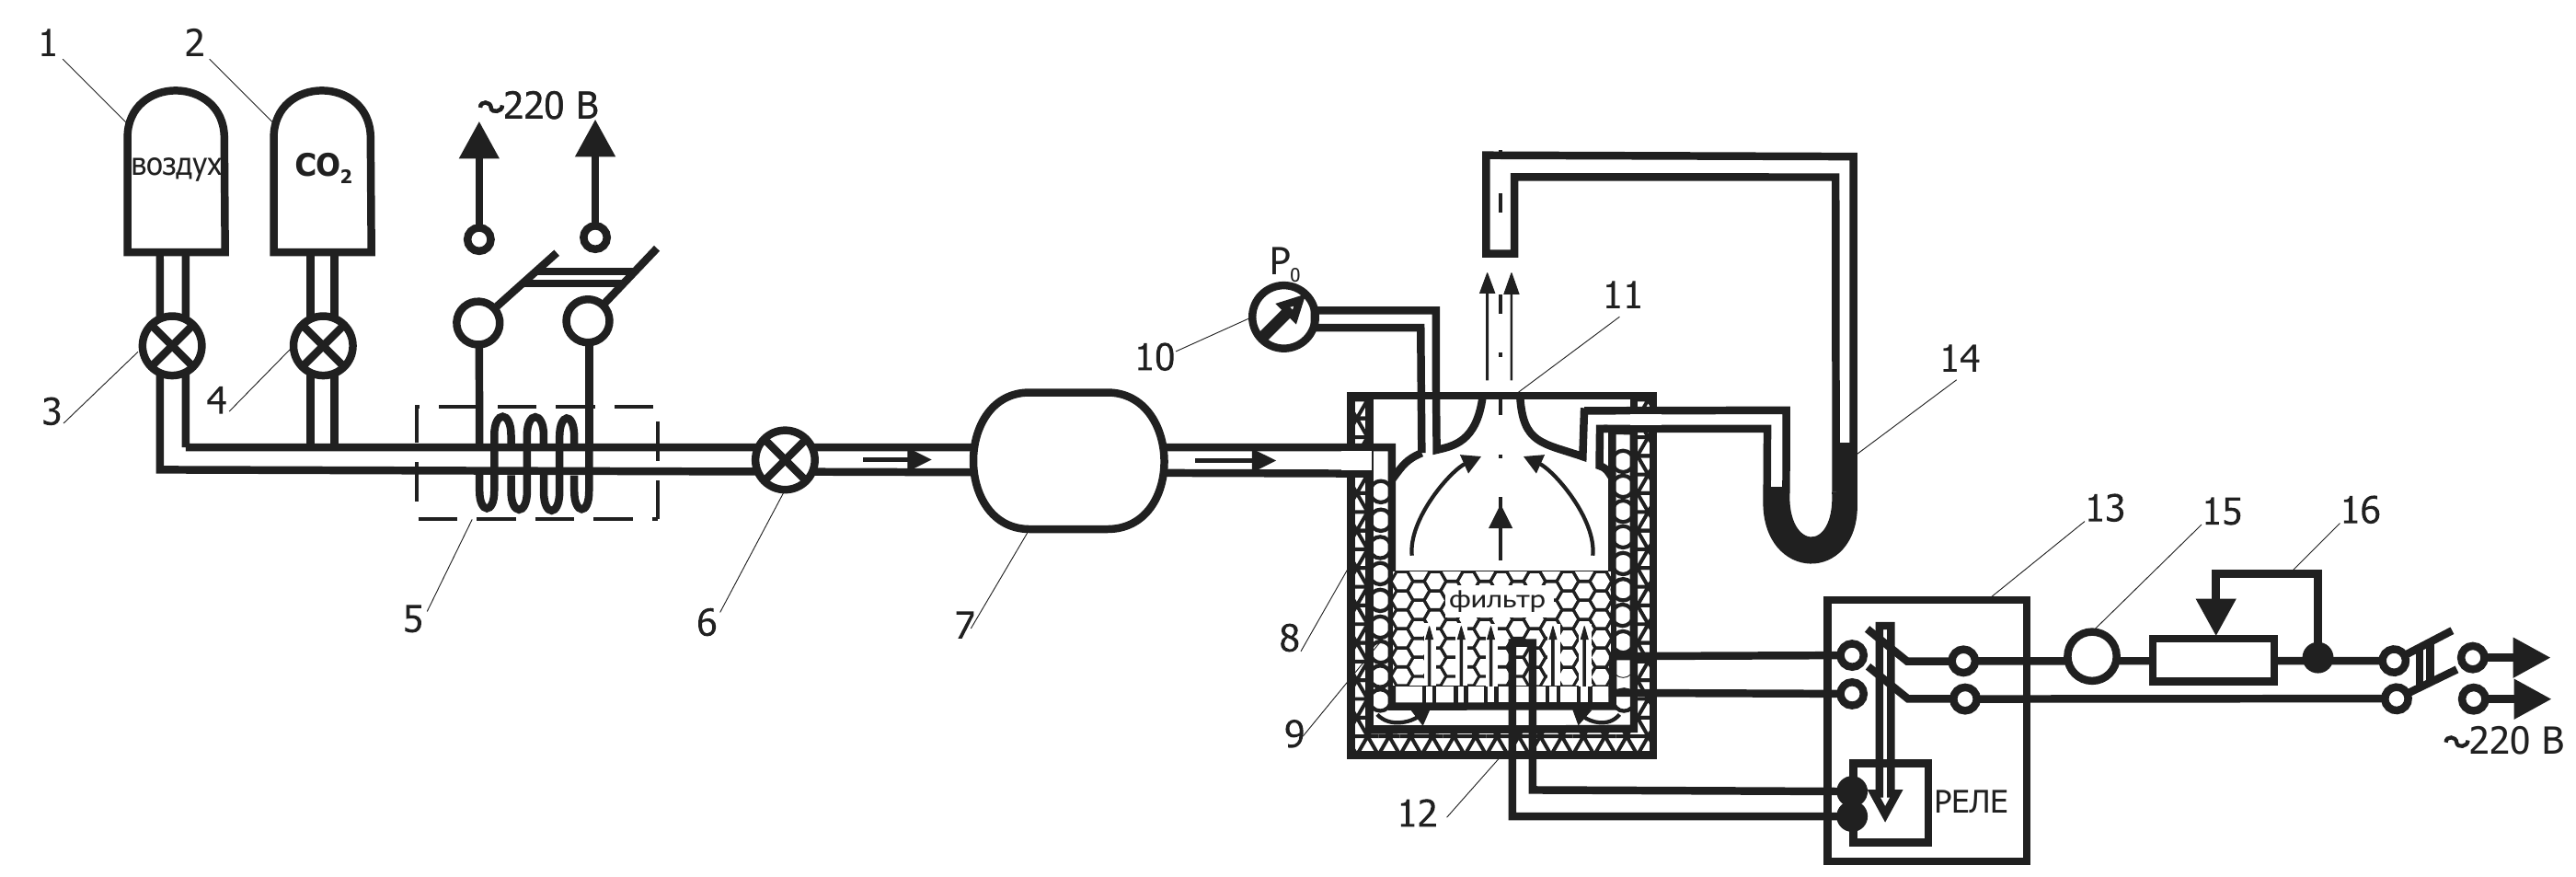
\includegraphics[width=0.77\textwidth]{fig13_6_setup.png}
\caption{Схема установки \cite[рис.~13.6]{labnik}. 9~--- подогреватель,
10~--- манометр ресивера, 11~--- ресивер с соплом, 12~--- термопара,
14~--- водяной дифманометр.}
\end{figure}

При быстром торможении колебательные степени свободы запаздывают
за нагревом газа. Последующее выравнивание температур увеличивает
энтропию и снижает полное давление. После полного торможения и
релаксации газ возвращается к $T_0$ по балансу полной энтальпии.
Для идеального газа измеренному перепаду соответствует
\begin{equation}
 \Delta S=-R\ln\left(1-\frac{\Delta p}{p_0}\right),
 \qquad R=188{,}9~\text{Дж/(кг$\cdot$К)}.
\end{equation}

Считая разгон в сопле изэнтропическим, находим температуру $T_1$
и скорость $V_1$ на срезе сопла по атмосферному давлению $p_1$:
\begin{equation}
 x=\frac{T_0-T_1}{T_0}=1-\left(\frac{p_1}{p_0}\right)^{R/c_p},
 \qquad V_1=\sqrt{2c_pT_0x}.
\end{equation}
Активная теплоёмкость $c_{pa}=7R/2$, колебательный вклад
$c_{vib}=c_p-c_{pa}$. В модели гармонических осцилляторов
$c_p=843{,}0$ и $884{,}2$~Дж/(кг$\cdot$К) при 24 и 65\,$^\circ$C.
Расчёт теплоёмкости и вывод максимума энтропии приведены в отдельном
файле с ответами на контрольные вопросы. Для мгновенного торможения
с последующей релаксацией этот максимум равен
\begin{equation}
 \Delta S_{\max}=-c_{pa}\ln\!\left(1+\frac{c_{vib}}{c_{pa}}x\right)
                 -c_{vib}\ln(1-x).
\end{equation}

По оцифрованному графику со стенда (рис.~\ref{fig:stand}) для
$\bar S=\Delta S/\Delta S_{\max}$ считываем $r=\tau_{VT}/\tau_h$,
где $\tau_h=c_pd/(c_{pa}V_1)$ и $d=1$~мм~--- наружный диаметр трубки Пито.
При оцифровке исправлена перспектива фотографии по рамке графика.
Между соседними отсчётами интерполируем $\lg r$. При $\bar S>1$
измерение выходит за предел модели.

\begin{figure}[H]
\centering
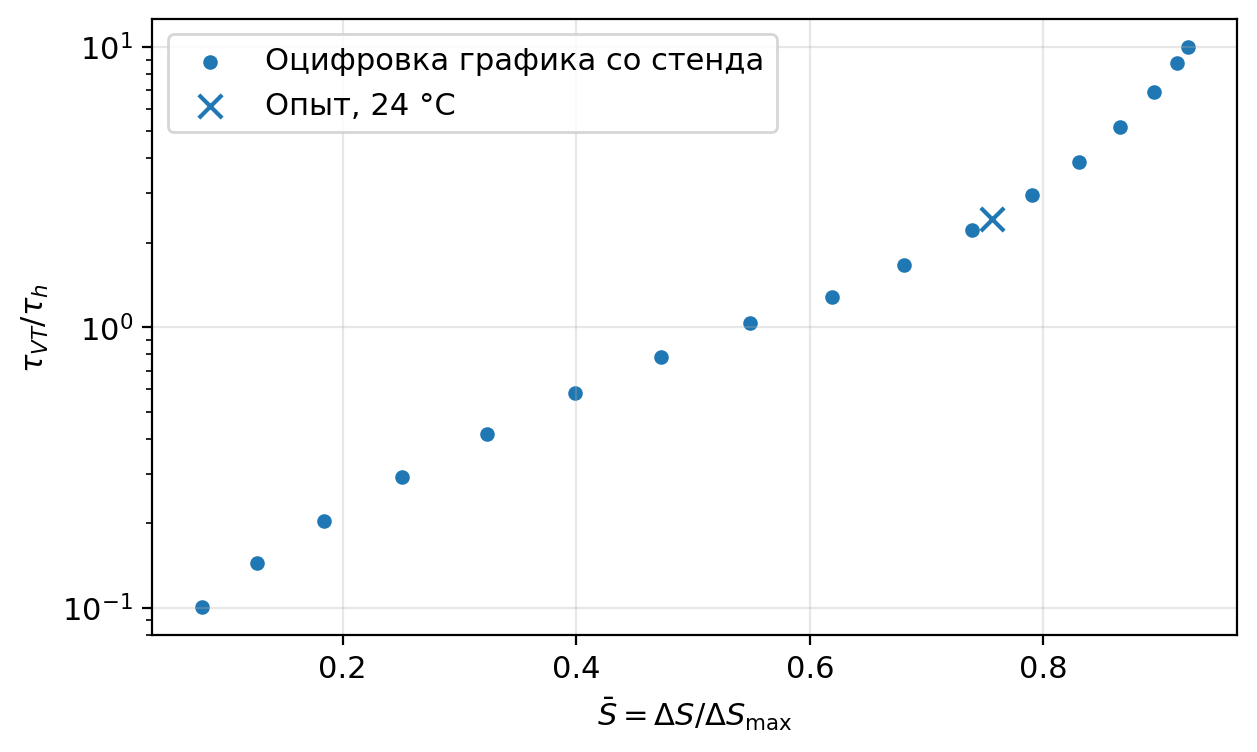
\includegraphics[width=0.48\textwidth]{entropy_curve.png}\hfill
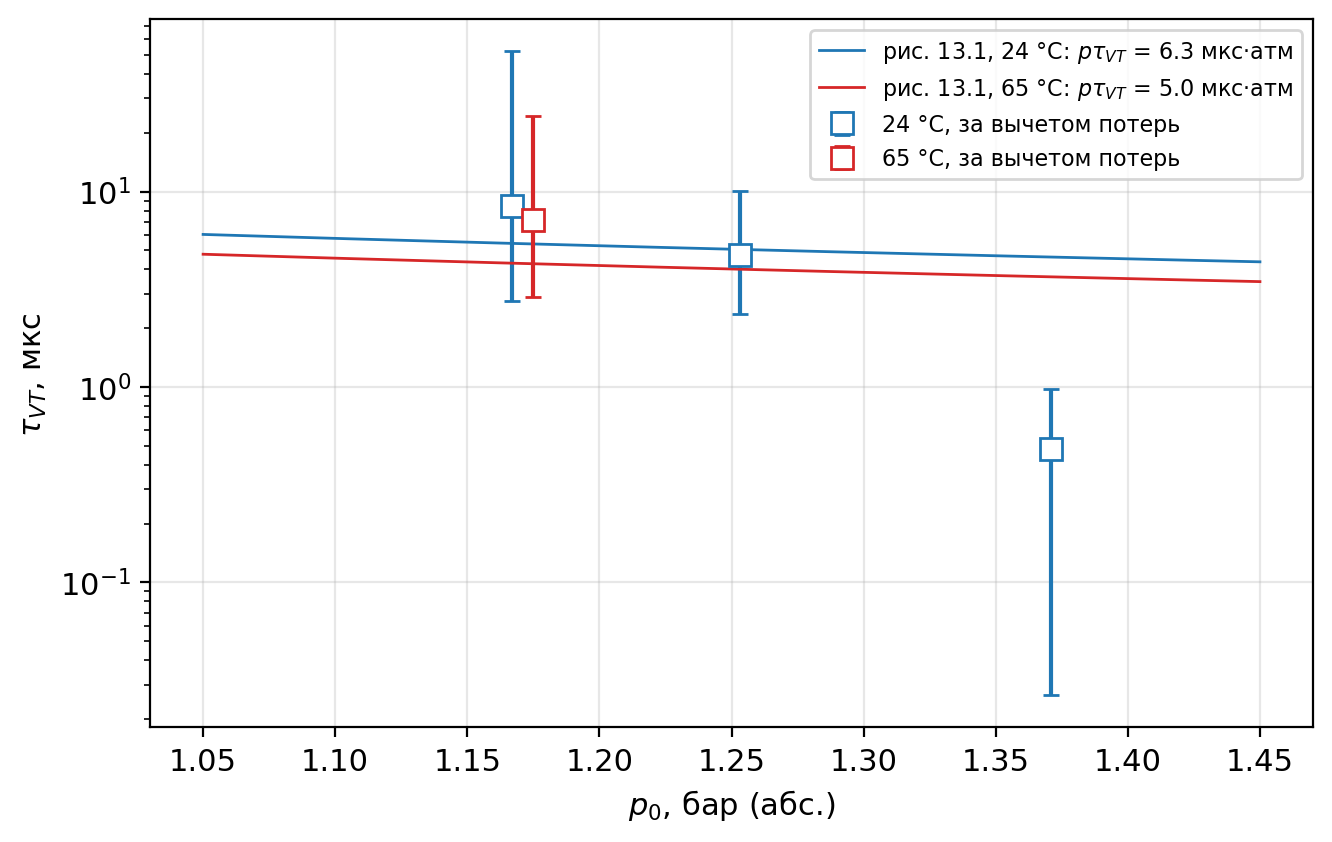
\includegraphics[width=0.48\textwidth]{tau_vs_p0.png}
\caption{Слева оцифрованный график со стенда с точкой опыта.
Справа время релаксации и справочные значения \cite[рис.~13.1]{labnik}.}
\label{fig:stand}
\end{figure}

\section{Измерения и результаты}

Атмосферное давление $p_1=740$~мм рт. ст. (98,66~кПа).
Для записанной в протоколе шкалы на 200 делений при пределе
1,6~кгс/см$^2$ получаем $p_0=p_1+784{,}5n$~Па, где $n$~--- число
делений. Записанная разность уровней воды $h$ соответствует
$\Delta p=97{,}8h$~Па при $h$ в сантиметрах. Перед сериями CO$_2$
проверили установку на воздухе: при $n=12$ получили 7~мм вод. ст.
при контрольном пороге 10~мм по практикуму. Далее измерили перепады
для двух температур при трёх давлениях в каждой серии.

\begin{table}[H]
\centering
\small
\setlength{\tabcolsep}{4pt}
\caption{Измеренные отсчёты и расчёт при 200 делениях на полную шкалу.
$\Delta S$ и $\Delta S_{\max}$ в Дж/(кг$\cdot$К).}
\begin{tabular}{rrrrrrrrrrr}
\toprule
$T_0$, $^\circ$C & $n$ & $h$, см & $\Delta p$, мбар & $p_0$, бар &
$x$ & $\Delta S$ & $\Delta S_{\max}$ & $\bar S$ & $V_1$, м/с & $\tau_h$, мкс \\
\midrule
24 & 23 & 2,0 & 1,96 & 1,167 & 0,0369 & 0,317 & 0,161 & 1,97 & 136 & 9,37 \\
24 & 34 & 3,2 & 3,13 & 1,253 & 0,0522 & 0,472 & 0,324 & 1,46 & 162 & 7,88 \\
24 & 49 & 3,4 & 3,33 & 1,371 & 0,0711 & 0,459 & 0,607 & 0,76 & 189 & 6,76 \\
\midrule
65 & 24 & 2,2 & 2,15 & 1,175 & 0,0366 & 0,346 & 0,203 & 1,70 & 148 & 9,03 \\
65 & 34 & 5,4 & 5,28 & 1,253 & 0,0498 & 0,798 & 0,379 & 2,11 & 173 & 7,74 \\
65 & 49 & 10,6 & 10,37 & 1,371 & 0,0679 & 1,434 & 0,709 & 2,02 & 201 & 6,64 \\
\bottomrule
\end{tabular}
\end{table}

Для точки при 24\,$^\circ$C и 49 делениях по графику $r=2{,}44$,
откуда $\tau_{VT}\approx16$~мкс. По рис.~13.1 практикума для этого давления
ожидается $4{,}6$~мкс. Изменение отсчёта $h$ на $\pm0{,}1$~см при прочих
равных даёт диапазон 15--19~мкс. В остальных точках $\bar S>1$.

\clearpage
\subsection{Проверка шкалы манометра}

При 100 делениях на тот же предел цена деления составила бы 1569~Па.
Результаты пересчёта приведены в таблице. Все шесть точек попадают
на ветвь графика, а при 23--24 делениях отклонение от справочных
данных меньше. При 49 делениях давление $1{,}73$~атм выходит
за рекомендованный предел $1{,}6$~атм. До проверки прибора
используем указанную в протоколе шкалу на 200 делений.

\begin{table}[H]
\centering
\caption{Проверочный расчёт для шкалы на 100 делений.}
\begin{tabular}{rrrrrr}
\toprule
$T_0$, $^\circ$C & $n$ & $p_0$, бар & $\bar S$ & $\tau_{VT}$, мкс &
$\tau_{VT}$ по рис.~13.1, мкс \\
\midrule
24 & 23 & 1,347 & 0,50 & 6,05 & 4,70 \\
24 & 34 & 1,520 & 0,38 & 3,11 & 4,17 \\
24 & 49 & 1,755 & 0,20 & 1,14 & 3,61 \\
65 & 24 & 1,363 & 0,44 & 4,51 & 3,68 \\
65 & 34 & 1,520 & 0,54 & 5,90 & 3,30 \\
65 & 49 & 1,755 & 0,53 & 4,89 & 2,86 \\
\bottomrule
\end{tabular}
\end{table}

\section{Оценка нагрева в ресивере}

Для подъёма температуры с 24 до 65\,$^\circ$C газу нужно передать
$q=c_p\Delta T\approx35$~кДж/кг. Для цилиндра диаметром 35~мм,
длиной 0,60~м и плотности CO$_2$ около 2~кг/м$^3$ тепловой баланс даёт
\[
 P_{\text{газ}}=\rho A u q\approx68~\text{Вт}\frac{u}{1~\text{м/с}},
 \qquad t=\frac{L}{u}.
\]
Например, при $u=0{,}5$~м/с получаем 34~Вт и 1,2~с.
При заданной передаваемой мощности нагрев уменьшается с увеличением
расхода. Время пребывания в этом примере намного больше времени
колебательной релаксации, поэтому колебания успевают прийти
к локальному равновесию. Для оценки фактического нагрева нужен
расход газа.

\section{Выводы}

Измерения дают одну оценку времени релаксации при принятой шкале
манометра. Расхождение со справочными данными может быть связано
с аппаратными потерями и погрешностями отсчётов. Для проверки
зависимости времени релаксации от температуры и давления нужны
уточнение шкалы и повторные измерения.

\begin{thebibliography}{9}
\bibitem{labnik} Физическая механика. Лабораторный практикум по газовой
динамике, гидродинамике и физической механике / под ред. Э.~Е.~Сона.
М.: МФТИ, 2004. Гл.~13.
\end{thebibliography}
\end{document}
